\documentclass[11pt, titlepage, a4paper]{article}

\usepackage{graphicx} % For images
\graphicspath{ {./graphics/} }
\usepackage[acronym]{glossaries}
\usepackage[automake]{glossaries-extra}
\usepackage[utf8]{inputenc} % For special characters
\usepackage[english]{babel} % For language-specific hyphenation patterns
\usepackage[hidelinks]{hyperref} % For clickable links
\usepackage{enumitem}
\usepackage[]{datetime2}
\usepackage[a4paper, total={17.5cm, 25cm}]{geometry}
\usepackage[backend=biber, style=ieee, sorting=none]{biblatex}
\addbibresource{Internship.bib} % Imports bibliography file+
\def\labelitemi{--}
\usepackage[T1]{fontenc}
\usepackage{inconsolata}
\usepackage{float}

\usepackage{color}

\definecolor{pblue}{rgb}{0.13,0.13,1}
\definecolor{pgreen}{rgb}{0,0.5,0}
\definecolor{pred}{rgb}{0.9,0,0}
\definecolor{pgrey}{rgb}{0.46,0.45,0.48}

\usepackage{listings}
\lstset{language=Java,
  showspaces=false,
  showtabs=false,
  breaklines=true,
  showstringspaces=false,
  breakatwhitespace=true,
  commentstyle=\color{pgreen},
  keywordstyle=\color{pblue},
  stringstyle=\color{pred},
  basicstyle=\ttfamily,
  moredelim=[il][\textcolor{pgrey}]{},
  moredelim=[is][\textcolor{pgrey}]{\%\%}{\%\%}
}



\title{Internship Report}
\author{Emily Sterthaus \\ Matriculation Number: 451 342 \\ \href{mailto:m_ster15@uni-muenster.de}{m\_ster15@uni-muenster.de}\\ \\
\small Ifgi Supervisor: \href{mailto:christian.knoth@uni-muenster.de}{Christian Knoth}\\ \small con terra Supervisor: \href{mailto:t.fechner@conterra.de}{Thore Fechner}
}
\date{\today}
\newcommand{\myparagraph}[1]{\paragraph{#1}\mbox{}\\}
\setcounter{secnumdepth}{5}
\setcounter{tocdepth}{5}
\makeglossaries
\newacronym{gd}{GD}{Geologischer Dienst}
\newacronym{exif}{EXIF}{Exchangeable Image File Format}
\newacronym{iptc}{IPTC IIM}{International Press Telecommunications Council Information Interchange Model}
\newacronym{csw}{CSW}{Catalogue Service for the Web}
\newacronym{dz}{DZ-Gefahr}{Digitaler Zwilling - Gefahr}
\newacronym{fme}{FME}{Feature Manipulation Engine}
\newacronym{thw}{THW}{Technisches Hilfwerk}
\newacronym{bhkg}{BHKG}{Gesetz über den Brandschutz, die Hilfeleistung und den Katastrophenschutz}
\newacronym{kritis}{KRITIS}{Kritische Infrastrukturen}
\begin{document}


\maketitle
\newpage
\tableofcontents
\newpage

\section{Introduction}

My Internship was done at the con terra Münster. It started 2023-09-01 and ended 2024-03-31.
\subsection{Company Profile}
con terra is a geo-IT company based in Münster, Germany. The company primarily develops customer-specific GeoIT solutions based on the \glsxtrfull{fme} and various Esri technologies, such as ArcGIS. For this reason, con terra is an Esri Platinum Partner and the main distribution partner of Safe Software for \glsxtrshort{fme}.

On this basis, con terra also offers its own products, such as map.apps and smart.finder. Each with several add-ons and configurations, for example smart.finder - SDI or map.apps ETL. As an alternative, they are also working on an open source framework called Open Pioneer.  %Todo: Hierüber muss ich drignend mit thore sprechen ob das so passt

The con terra works with multiple different companys and governmental Organizations, such as TenneT TSO,  \glsxtrfull {gd} NRW, IT.NRW or the Bundesanstalt für Geowissenschaften und Rohstoffe  (BGR).

\subsection{Motivation}
As a Master’s student specializing in Geoinformatics and Spatial Data Science, my internship at con terra represents a strategic step in my professional development. Given my previous work experience with the company, I am already familiar with its standing as a leading geospatial software provider in Münster. This familiarity allows me to integrate seamlessly into the team and contribute effectively from the onset. The focus of the internship on software development is in perfect harmony with my academic training, promising a direct application of theoretical knowledge in a practical setting. My objective during this internship is to further refine my software development skills, leveraging the opportunities at con terra to enhance my technical expertise in geospatial IT

\section{Internship Content}

My internship was clearly structured. This took the form three different Projects, each in their own timeframe and with their own requirements.

\subsection{Geologischer Dienst NRW - Metdata Asset Managment System}
\subsubsection{Introduction}
The  \glsxtrshort {gd} NRW has a large achieve of different assets, which are currently managed by a software named cumulus. As the used software is outdated, it does not meet the the current requirements.
Primarily they  are required to make all data, where it is legally possible, open data \cite{GesetzZurForderung2017}.
Additionally the GeolDG also requires the \glsxtrshort{gd} to make their accessible by the public \cite{GesetzZurStaatlichen2020}.

Therefore, the main goal of this project was to conceptualize a new system and to implement parallel a prototype of it.
\subsubsection{As-is Status}
The \glsxtrshort{gd} digital archive contains over 450,000 assets. Assets in this context are for example images, PDFs, TIFs or MP4s. However, any digital file can be an asset. The total data volume is over 2 terabytes.
These assets are currently located on a shared drive and can be managed via the file system. They also use a piece of software called Cumulus. This software primarily manages the metadata associated with the assets. Currently, the \glsxtrshort{gd} does not use any known metadata schema, but instead uses a list of custom attributes, such as Rating, Special Instructions and Label.
They also use \glsxtrshort{exif} and \glsxtrshort{iptc} metadata information for images, which is not managed by Cumulus. Instead, this is done with an additional software component. %Likely Irfanview 

\subsubsection{The new system}
The new system exists maninly as a concept. But a few features were already implemented as a prototype for the \glsxtrshort{gd} to test them.
\myparagraph{Requirements}
The new system should eliminate the inadequacies of the old system. Therefore a list of Requirements were collected. In the following there is a subset example of the main functional requirements:
\begin{itemize}
	\item Keeping the Internal metadata attributes (and adding new ones)
	\item Connection to the GEOportal.NRW
	\item CRUD Operations for Datasets and associated metadata
	      \begin{itemize}
		      \item With an Integrated Permission System for Internal (\glsxtrshort{gd} Employees) and Externals
		      \item (Multi-)Edit Interface for Metadata
	      \end{itemize}
	\item Sharing data
	\item Update \glsxtrshort{exif} and \glsxtrshort{iptc} when an update occurs
	\item Syncing/Translating Internal Metadata to ISO 19115/ISO 19119
	\item Different Search Operations
\end{itemize}


\begin{figure}[t]
	\caption{Use case diagram, which visualized some functional requirements}
	\label{fig:usecase}
	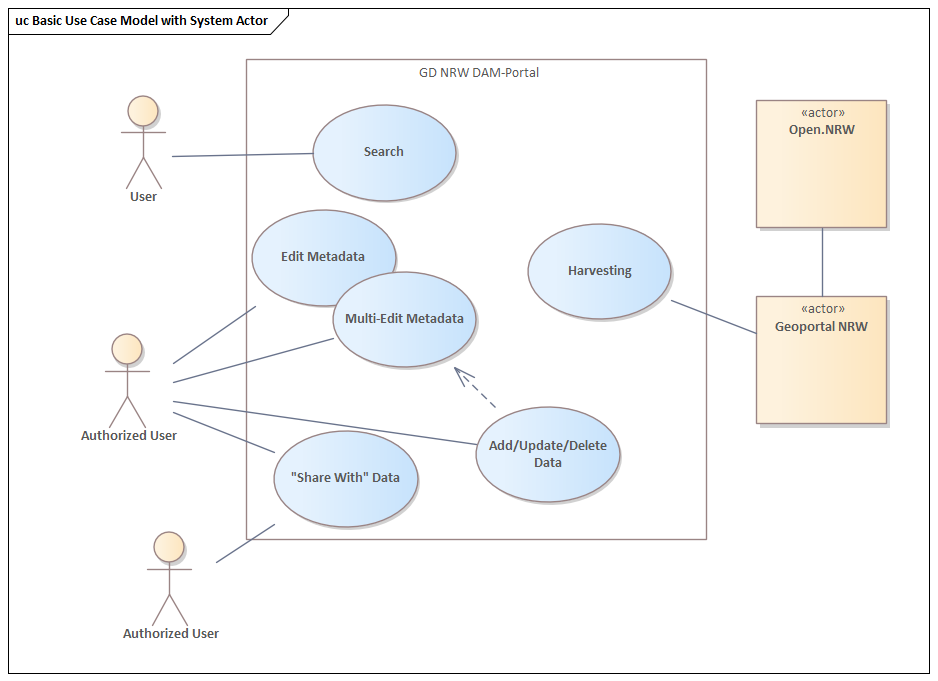
\includegraphics[width=16cm]{usecase_diagramm.png}
	\centering
\end{figure}

In addition, there are a number of quality requirements that focus primarily on data integrity and the tech stack used for development. For example, the software developed should be able to live in the cloud or on a dedicated machine.

A final requirement is that the system needs to be split. It should mainly run on the servers of IT.NRW. But only non-sensitive data should be hosted there. Sensitive data should be hosted and only accessible by the \glsxtrshort{gd} and its staff.

\myparagraph{Implementation}
To meet these Requirements the smart.finder SDI was choosen as base software. As it can not meet all requirements standalone (for example it can only work with ISO 19115/ISO 19119, INPSIRE or GDI DE Metadata) new software components were conceptualized and implemented to meet the designated requirements.

\begin{figure}[t]
	\caption{Planned software components (partial abstracted)}
	\label{fig:components}
	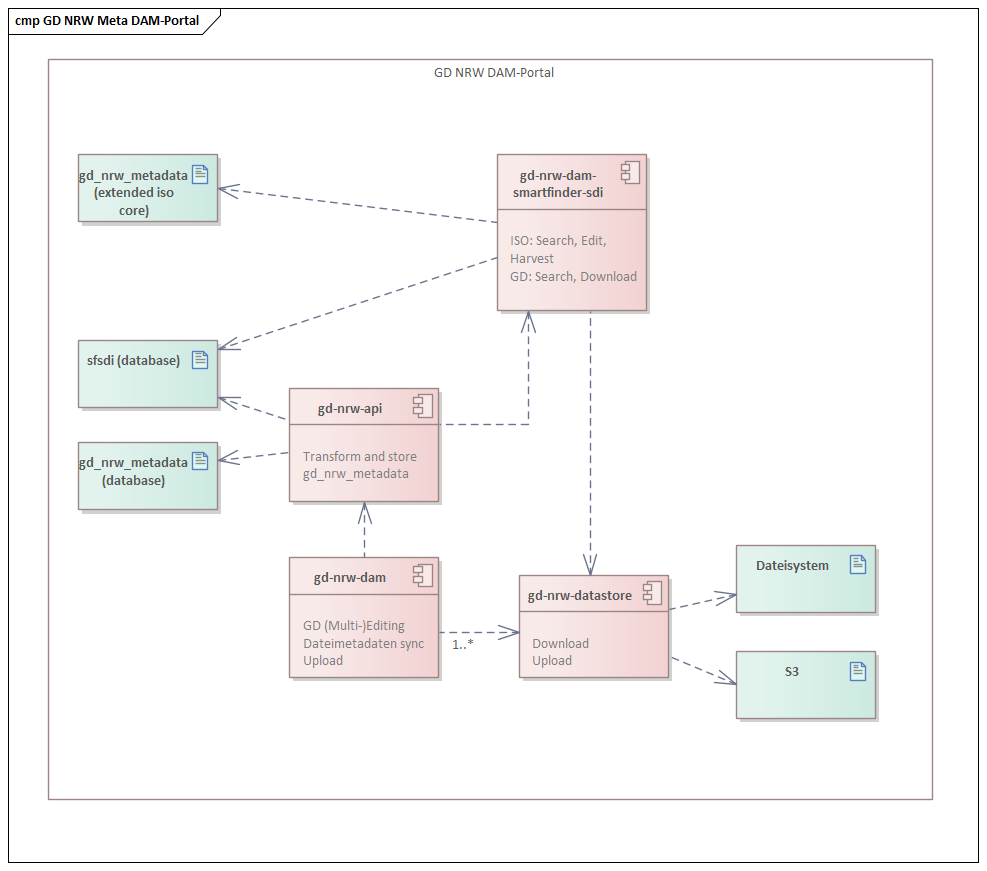
\includegraphics[width=16cm]{components.png}
	\centering
\end{figure}

As seen in \ref{fig:components} the new Software consists of a gd-nrw-api, gd-nrw-dam-smartfinder-sdi, gd-nrw-dam and gd-nrw-datastore.
In the following each software component will be shortly described:
\begin{description}[]
	\item[gd-nrw-dam-smartfinder-sdi]: This represents the smart.finder SDI, comprising several software components, including the smartfinder-search, smartfinder-editor, smartfinder-csw and smartfinder-sdi, as well as the gd-nrw-dam-portal.
	      \begin{description}[]
		      \item[smartfinder-search]: This component is responsible for managing data. It operates on an integrated Apache Solr instance to enable the search and filter capabilites of the smartfinder. It also enables features such as full-text search, geo-searches, and filtering for specific attribute values.
		      \item[smartfinder-editor]: This component represents the smart.editor, which enables the editing of Metadata in compliance with ISO 19115/ISO 19119, INSPIRE, or GDI DE.
		      \item[smartfinder-csw]: This component serves as the \glsxtrshort{csw} interface, enabling the dissemination of data to other portals, including the GEOportal.NRW.
		      \item[smartfinder-sdi]: This component constitutes the user interface for searching and accessing datasets.
		      \item[gd-nrw-dam-portal]: This component is an adapted version of the smartfinder-sdi component.
	      \end{description}
	\item[gd-nrw-dam]: This component offers CRUD functionality for metadata, including a frontend for Multi-Edit Metadata and Editing Single Metadata.
	\item[gd-nrw-datastore]: This component is responsible for the raw data access. It has the ability to function with both the raw file system and S3 Storages. It offers fundamental CRUD capabilities for the data.
	\item[gd-nrw-api]: This component stores the metadata and manages the communication between the newly developed software components and the smartfinder-sdi.
\end{description}
The general workflow for documents is that all editing is done by \glsxtrshort{gd} Staff, therefore their component handle all editing.

As the GD wanted to keept its own Metadata scheme, an additional database was required to save these Attributes.  This database  is called gd-nrw-metadata. Its schema special developed to not allow any M-N relationships, as this was required.  The schema is visible in \ref{fig:db}.


\begin{figure}[t]
	\caption{Planned Deployment Diagramm}
	\label{fig:deployment}
	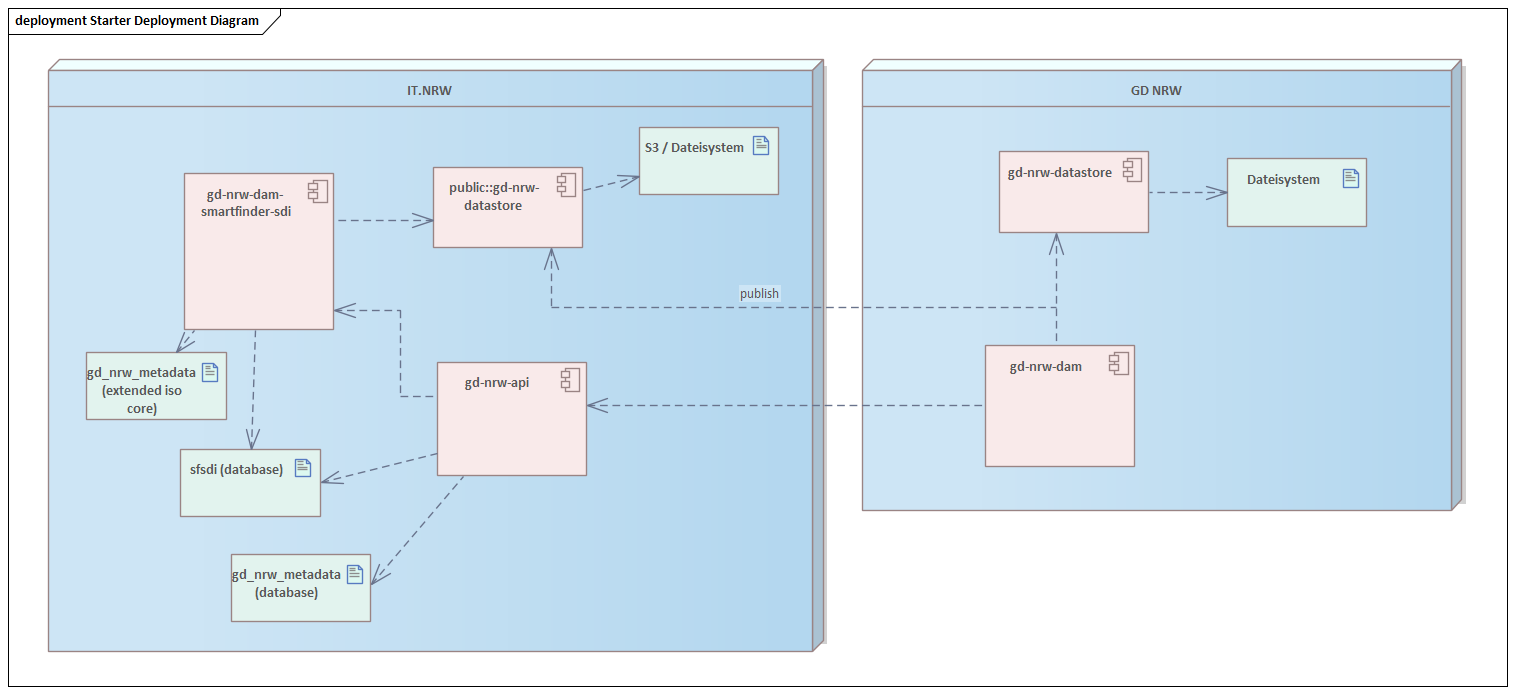
\includegraphics[width=16cm]{deployment.png}
	\centering
\end{figure}

As part of the planning, a deployment diagram was created, figure \ref{fig:deployment}. To achieve the goal of splitting the data between two hosts, there are now two datastores that can be switched in place. This is necessary to allow authorised users to access sensitive data. The metadata is still completely hosted by IT.NRW, but can be locked behind a login and is therefore not available to the public. The aim of this configuration is to duplicate as few services as possible.
An alternative was to build a complete clone system for IT.NRW and \glsxtrshort{gd} and only synchronise the open access datasets.

\subsubsection{My Participation}
My involvement in this project focused on the development of new software components for a prototype. Furthermore, I made modifications to the smartfinder-sdi.

\begin{figure}[t]
	\caption{Database Scheme}
	\label{fig:db}
	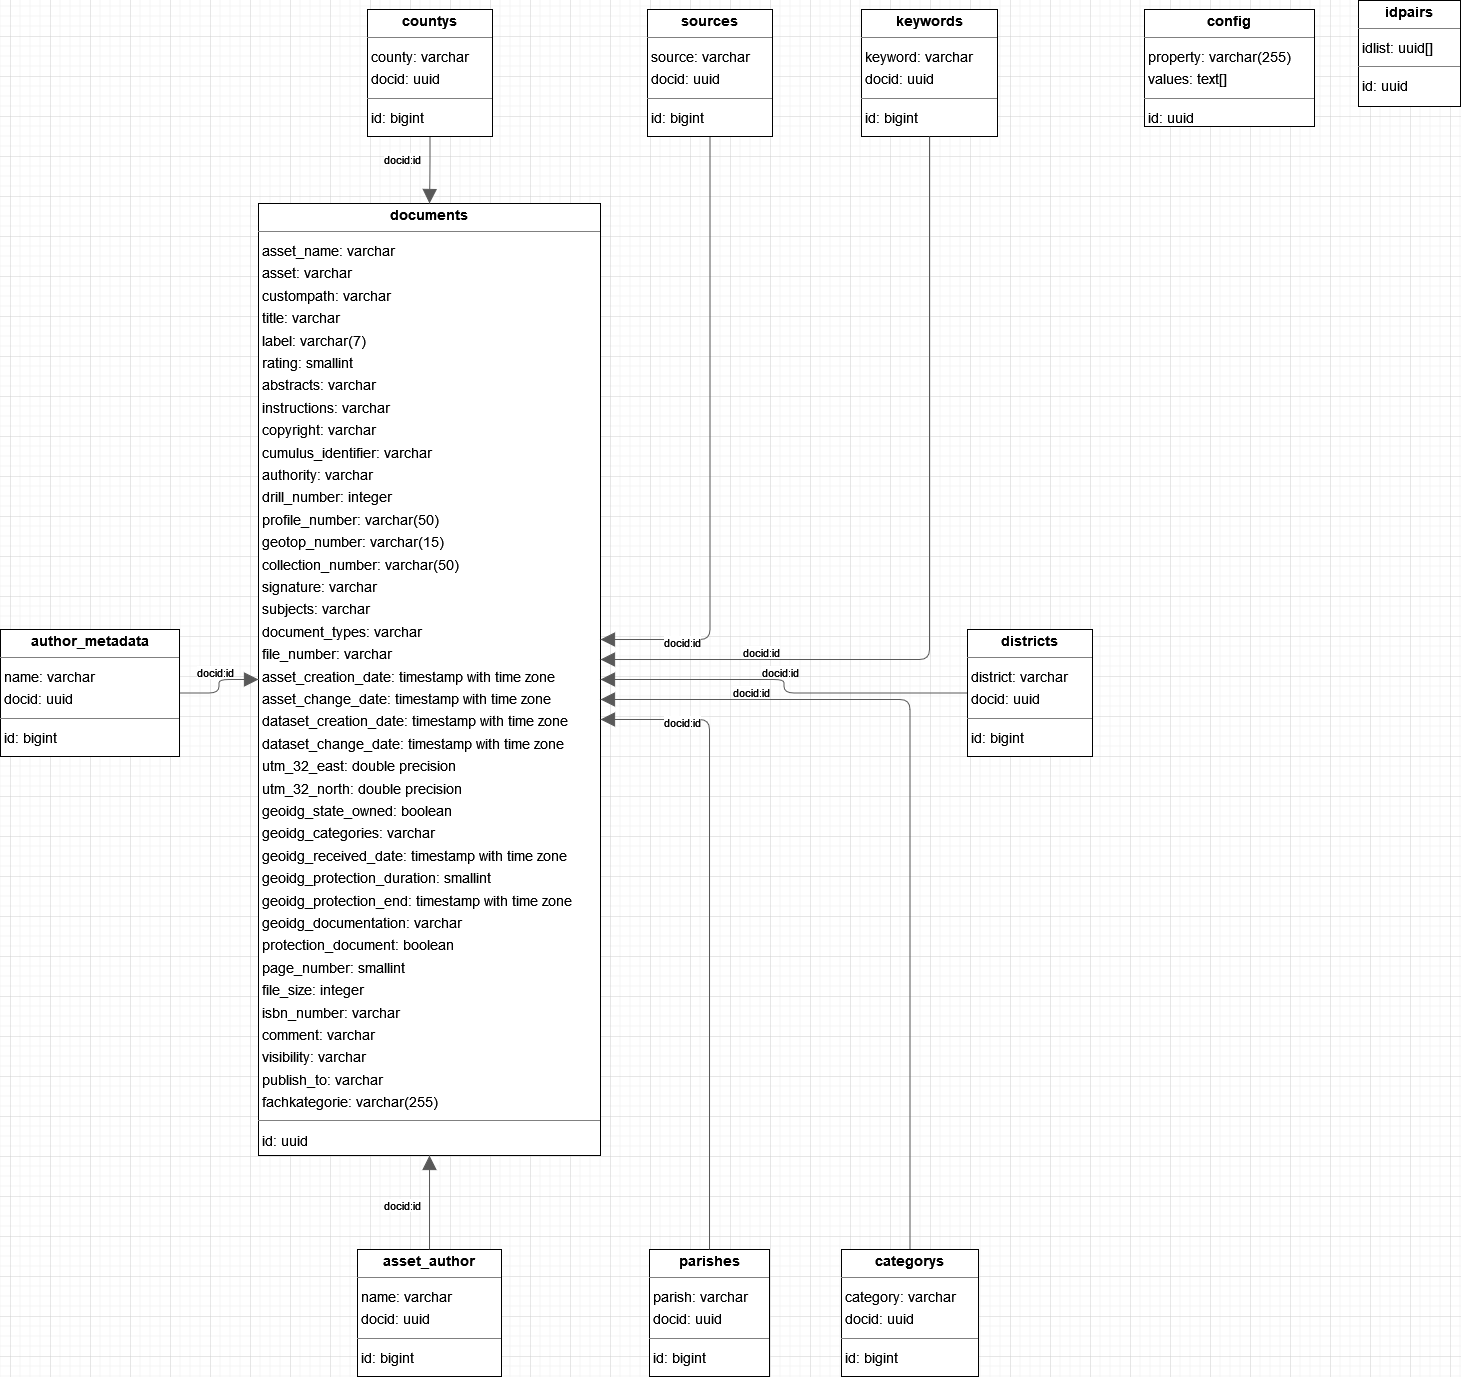
\includegraphics[width=16cm]{db3.png}
	\centering
\end{figure}

The initial prototype commenced as a basic project employing FastAPI and Python. It also integrated an added PostgreSQL database. The principal objective was to construct a database schema tailored to our requirements. The final configuration is depicted in Graphic \ref{fig:db}. We opted for a flat structure with no N-M relationships. 
Also, I designed the frontend. Our technological stack for the frontend consisted of Vue and Vuetify, with the inclusion of a Vite development server. The primary Vue components that I developed include Single Editing for modifying a single Metadataset and Multi-Edit for modifying multiple Metadatasets. To create Single Editing, I used a mockup as a template to base my development on. I designed and conceptualised Multi-Editing myself, as demonstrated in figure \ref{fig:multiedit}.  

Later on in the project, I developed an additional front-end for a shopping cart, which serves as an intermediary website between the Smartfinder and the new components. Moreover, I developed a front-end for the administrator to configure various attributes for editing.

\begin{figure}[t]
	\caption{Screenshot MultiEditing}
	\label{fig:multiedit}
	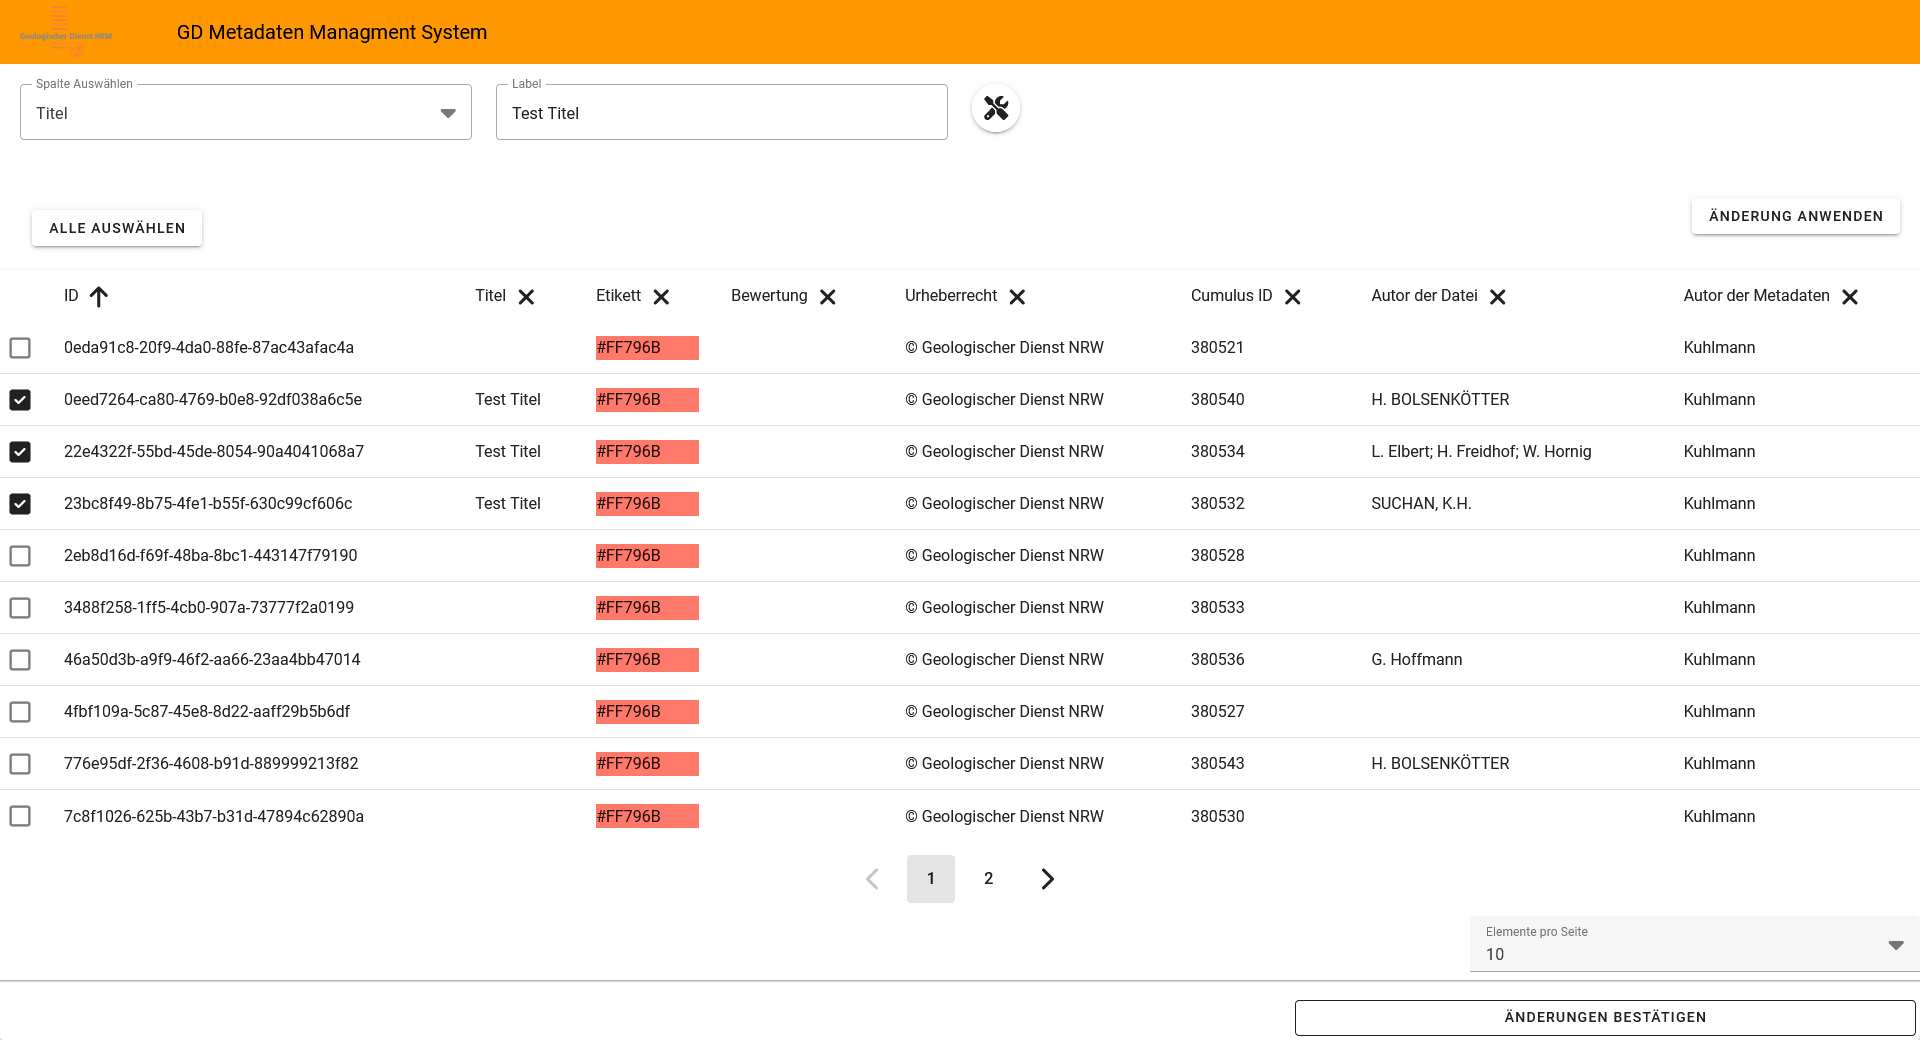
\includegraphics[width=16cm]{multiedit.png}
	\centering
\end{figure}
\begin{figure}[t]
	\caption{Vue Java Controller}
	\label{fig:vue}
	\begin{lstlisting}[language=java, frame=single]
        @Controller
        public class VueController {
            @RequestMapping(value = "/*/{path:[^\\.]*}")
            public String redirect(){
                return "forward:/";
            }
        
        
        }
        
        \end{lstlisting}
	\centering
\end{figure}


After that, a decision was made to drop Python and FastAPI in favour of Spring Boot and Java. Therefore, I have commenced composing the gd-nrw-dam module. The gd-nrw-datastore module is integrated into the prototype of the gd-nrw-dam module. This began by implementing the required Spring Data classes and interfaces, followed by Afterwards, I began implementing the fundamental endpoints for CRUD operations to restore functionality to my frontend. Additionally, the capacities to host the built front-end on the Spring Boot server were incorporated. I developed a special Spring Boot controller to keep the Vue router component of the frontend working, as it controls the routing for which page is loaded. The code for this can be found in \ref{fig:vue}. It should be noted that any requests that match the applied regex pattern will be directed to the Vue Router. 

Following that, I developed an Azure build pipeline for automated deployment on our test system.  To achieve this, I restructured the project into two separate components: the frontend and the backend, each with its own pom.xml file. Additionally, there is a pom file for the entire project, enabling Maven to build the project with the complete frontend included in the backend for the pipeline. The tomcat-maven-plugin was then used for deployment to our test machine.

Later, I developed the Sfsdi API component, which serves as a predecessor to the gd-nrw API. It is a Spring Boot application that accesses the Smartfinder-Search module and alters its Solr database. During development, I extended the smartfinder-search Solr core to handle additional data types beyond ISO. Moreover, I enhanced the frontend of the smartfinder-sdi, effectively creating the gd-nrw-dam-portal component.
Also i created an automated ISO XML generation.

Finally, I have developed several complex features, including thumbnail generation for images and PDFs, on-the-fly zipped group downloads, \glsxtrshort{iptc}/\glsxtrshort{exif} read and write capabilities, and the deployment of a Redis Instance for fast and secure storage. These addition will facilitate the transition from the smartfinder to the new components. Also i deployed an Nginx instance as a reverse proxy for basic authentication, with TLS support. 



\subsection{\glsxtrfull{dz}}
\subsubsection{Introduction}
After the flood disaster in the Ahrtal it was recognized that the hazard prevention and emergency response in the federal state NRW is not optimal. Dispatched units, e.g. \glsxtrshort{thw} and fire department, could not really comunicate and organize their actions. But communication and organization is a key part, as it allows effiecient and fast responses. 
After the "Krisenbewältigungsgesetz" in NRW was deployed on December 2022, it was decided that this lack of competence is an emergency situation on February 23. To solve this there was an budget of 500.000€ provided.
The con terra applied together with IT.NRW to develop a solution to this problem.
The solution of the con terra is a digital twin with the focus on aggregating all relevant data and visualize it optimally for each possible Scenario.  It should incorporate multiple relevant datasets from multiple sources. Source system in this context are for example the GDI-NW, the LVN and the Bund BKG.


\subsubsection{As-is Status}
There are currently no central systems in place to handle this kind of task. Mostly there are department specific solutions or even general purpose Systems like QGIS or ArcGIS.



\subsubsection{Requirements}
As this is an consulting project, with the main goal of develop an prototype, there are few hard requirements for it. Also a few of the requirements where also evaluated and set during the project in cooperation with fire departments. An excerpt of the main requirements for this project are the following: 


\begin{description}[]
	\item[3 Dimensionality]: As the real world is and its associated problems are 3 Dimensional the solution should acknowledge this. Therefore it should have the capabilities to visualize 3D Data and run simple general purpose processes like measurements on it. 
	\item[Scenario Optimized Geodata]: The digital twin should optimize it data visualization and access for different scenarios, as not each scenario can use each dataset. Main scenario Groups are here: Fire, Earth, Water, Air.
	\item[Follow the \glsxtrshort{bhkg}]: The prototype should be developed with the aim of planning / monitoring / follow-up in accordance with \glsxtrshort{bhkg}.
	\item[Target Group - Authorities and organizations with security tasks]:  The Prototype should be developed with its target group in mind, as it can not be expected that everyone has Geo specific knowledge 
	\item[Cloud based]: The complete application should live and run in the cloud.
	\item[Fine grained right concept]: As the application may contain critical data (e.g.,\glsxtrshort{kritis} data) it should have a right concept, so that each user can only access datasets relevant for them. 
	\item[Analysis tools]: The application should also provide extensive analysis tools. For the prototype this will be: Identify protected assets and analyze its accesibility, determine dynamically the waterlevel in 3D, Simulating spread of a smoke cloud in 3D.
	\item[Incoorporate 3D Meshes]:  The state of NRW is currently working on creating a detaield 3D mesh for the entire federal state. The digital twin should incorporate the complete dataset.
	\item[EPSG: 25832] As a governmental project, the entire application must use EPSG: 25832
\end{description}

But not all requirements will be full filled in this project!

\section{Implementation}
The project used as a base mapapps and was in an agile manner developed. From the requirements just a few were implemented.

\section{My Participation}
I came in the project shortly before it ended. Therefore i only fulfilled only a few tasks.
My main focus was on integrating fire department data, we were provided with. I was given a PEI Dataset. This dataset consisted of radio messages transmitting location data. Either Short PDU, Long PDU or STATUS. An example is visible in in \ref{fig:pei}. There first line contains metadata about the message, e.g., transmitting party, receiving party and message type.
The following HEX-Code can be translated to binary, which in turn can be now decoded accordingly to ETSI TS 100 392-18-1. I developed a simple python script which automated this task and outputs an ESRI feature layer.  
\begin{figure}[H]
	\caption{Fire department data entry}
	\label{fig:pei}
	\begin{lstlisting}[frame=single]
        +CTSDSR: 108,262100112345678,1,262100188888888,1,88,1
		0A004C9CD24739C9384820

        
        \end{lstlisting}
	\centering
\end{figure}

I also developed an new map control tool, which allows users a more intuitive way to control the position, rotation, tilt and zoom of  the map. The rotation in this case can be changed by dragging the north arrow and rotate it around the circle, as seen in \ref{fig:mapcontrol}.
\begin{figure}[H]
	\caption{Screenshot MapControl}
	\label{fig:mapcontrol}
	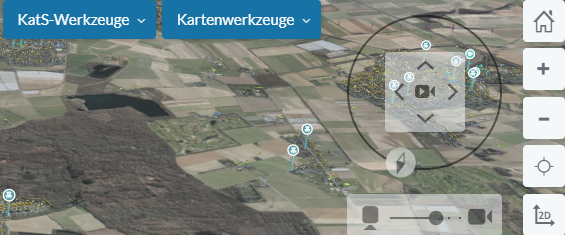
\includegraphics[width=16cm]{dzgefahr_mapcontrol.png}
	\centering
\end{figure}

I also enabled smooth Animations of moving objects in mapapps. This was espesecially inteded for a layer which displays the live position of each bus in Münster. Before that the Bus teleported every few meters. With my update the bus now mooves smoothly during a position update. This was done with the help of an third party library called animejs. 

Finally i evaluated how compatible Esris ArcGIS Indoors Technology is with mapapps. The result is that the 
compability is currently limited. 
\section{Reflection}

\clearpage
\printglossary[type=\acronymtype]
\printglossary
\clearpage
\printbibliography

\end{document}
